\documentclass{beamer}

\usepackage[czech]{babel}
\usepackage[utf8]{inputenc}
\usepackage{multicol}
\usepackage[backend=bibtex, style=iso-numeric, alldates=iso]{biblatex}

\usetheme{Madrid}
\definecolor{UBCblue}{rgb}{0, 0.698, 0.674}
\usecolortheme[named=UBCblue]{structure}

\title[Semestrální práce]{Vyhledávání K nejbližších sousedů na základě filtru}
\subtitle{Search K nearest neighbors based on a filter}
\author[Bc. Jan Jedlička, JED0050]{Bc. Jan Jedlička \\ {\footnotesize Vedoucí: Doc. Ing. Radim Bača, Ph.D.}}
\institute[]{FEI, VŠB-TUO}
\date{2022}

\titlegraphic{
\includegraphics[scale=0.2]{figures/vsb logo.jpg}}

\addbibresource{citace.bib}

\begin{document}
	
	\frame{\titlepage}
	
	\begin{frame}
		\frametitle{Úvod}
		
		\begin{itemize}
			\item Porozumění HNSW
			\item Vlastní HNSW implementace nebo zprovoznění jiné HNSW implementace
			\item Návrh a implementace rozšíření HNSW o filtr (podmínka, která stanoví, které vektory se při prohledávání vynechají)
		\end{itemize}
		
	\end{frame}

	\begin{frame}
		\frametitle{KNN}
		
		\begin{itemize}
			\item Vyhledávání K nejbližších sousedů od dotazu Q v n dimenzionálním prostoru
			\item Vzdálenost mezi body v prostoru definována metrikou (Euklidova, Hammingova, Minkowského atd.)
			\item U velkých dimenzí je pro většinu technik rychlejší sekvenční průchod
			\item Přibližné vyhledávání (ANN)
			\item Porovnávání vektorizovaných dat, hledání shluků, podobných vlastností (například vyhledávání sémanticky podobných dokumentů)
		\end{itemize}
		
	\end{frame}

	\begin{frame}
		\frametitle{KNN}
		\begin{figure}
			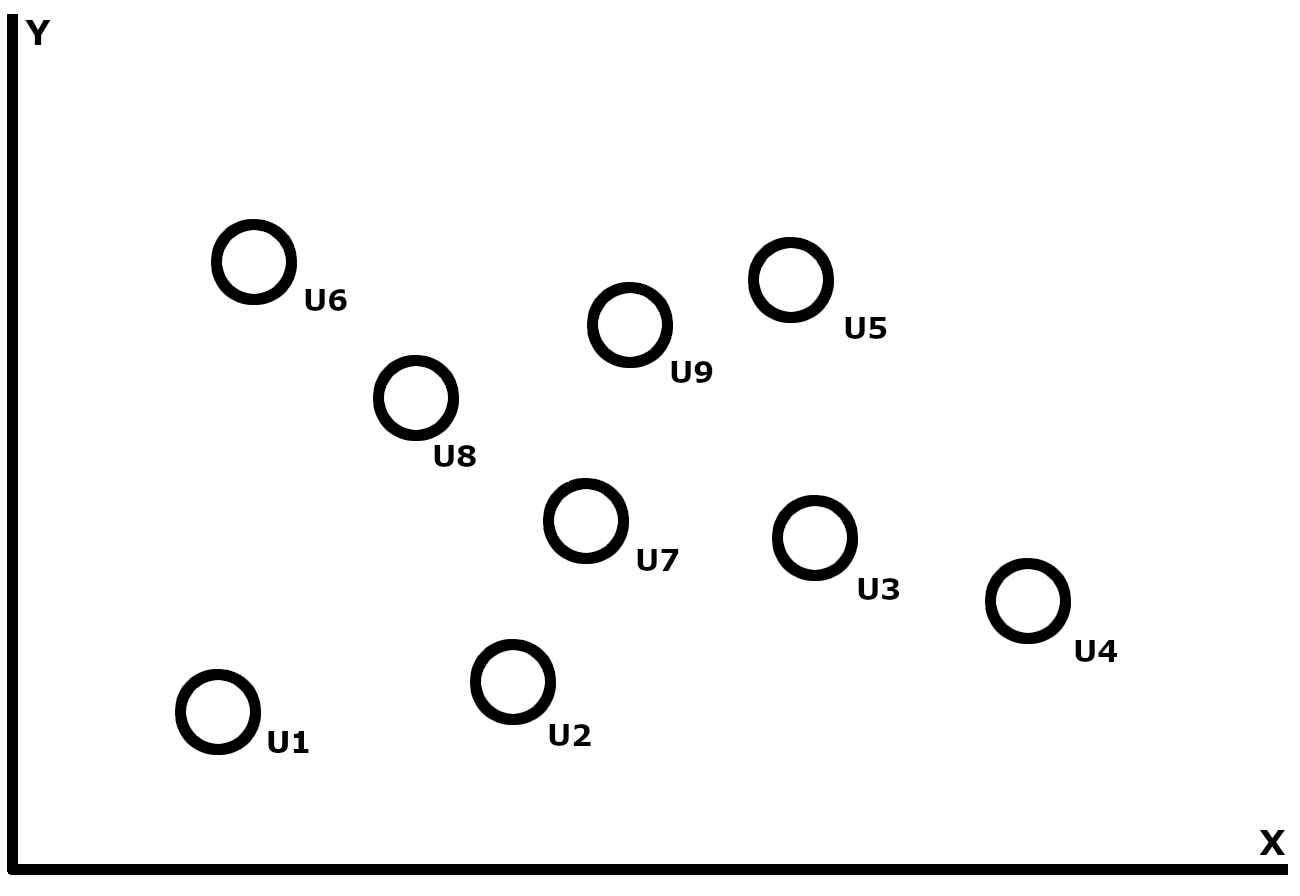
\includegraphics[scale=0.2]{figures/KNN_b1.jpg}
		\end{figure}
	\end{frame}
	
	\begin{frame}
		\frametitle{KNN}
		\begin{figure}
			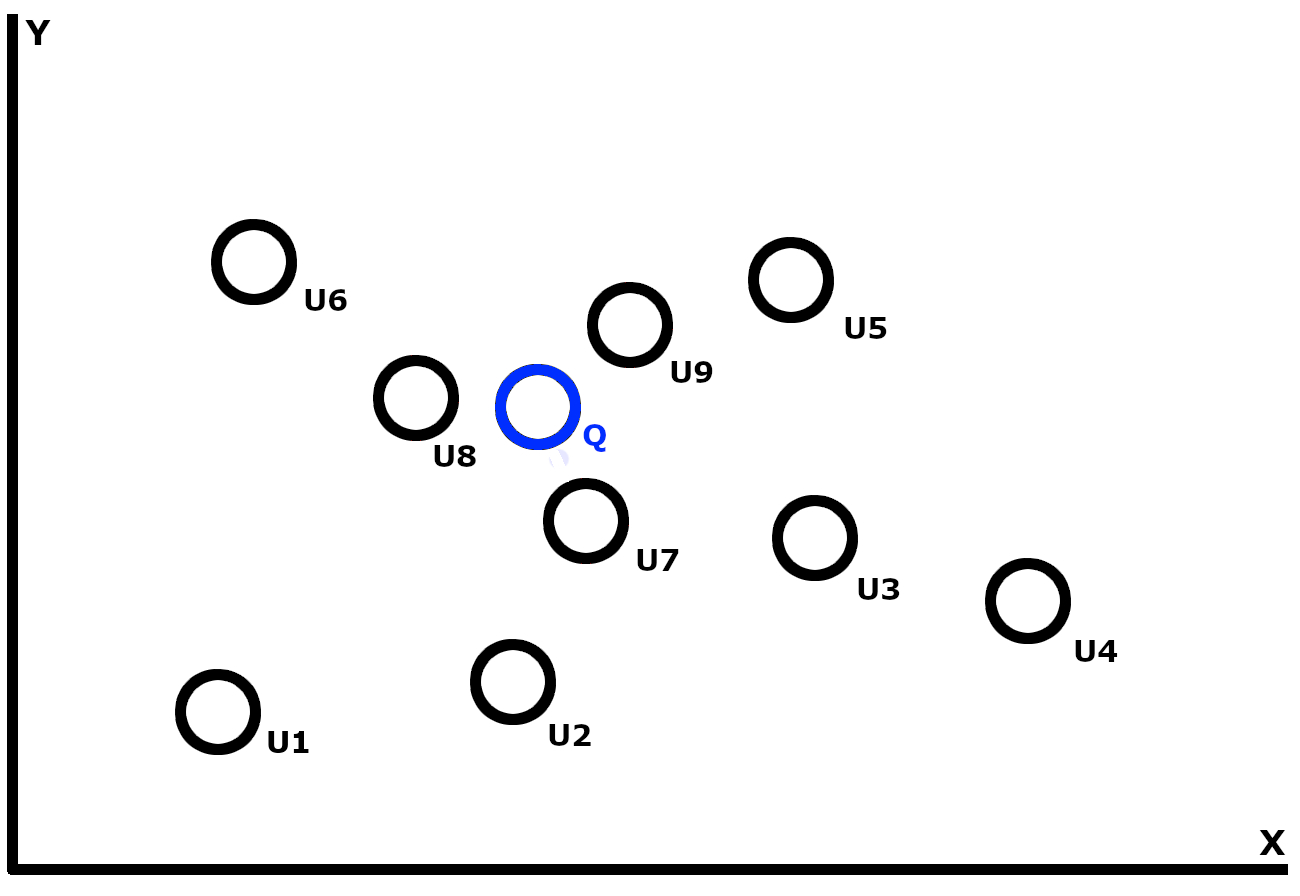
\includegraphics[scale=0.2]{figures/KNN_b2.jpg}
		\end{figure}
	\end{frame}

	\begin{frame}
		\frametitle{KNN}
		\begin{figure}
			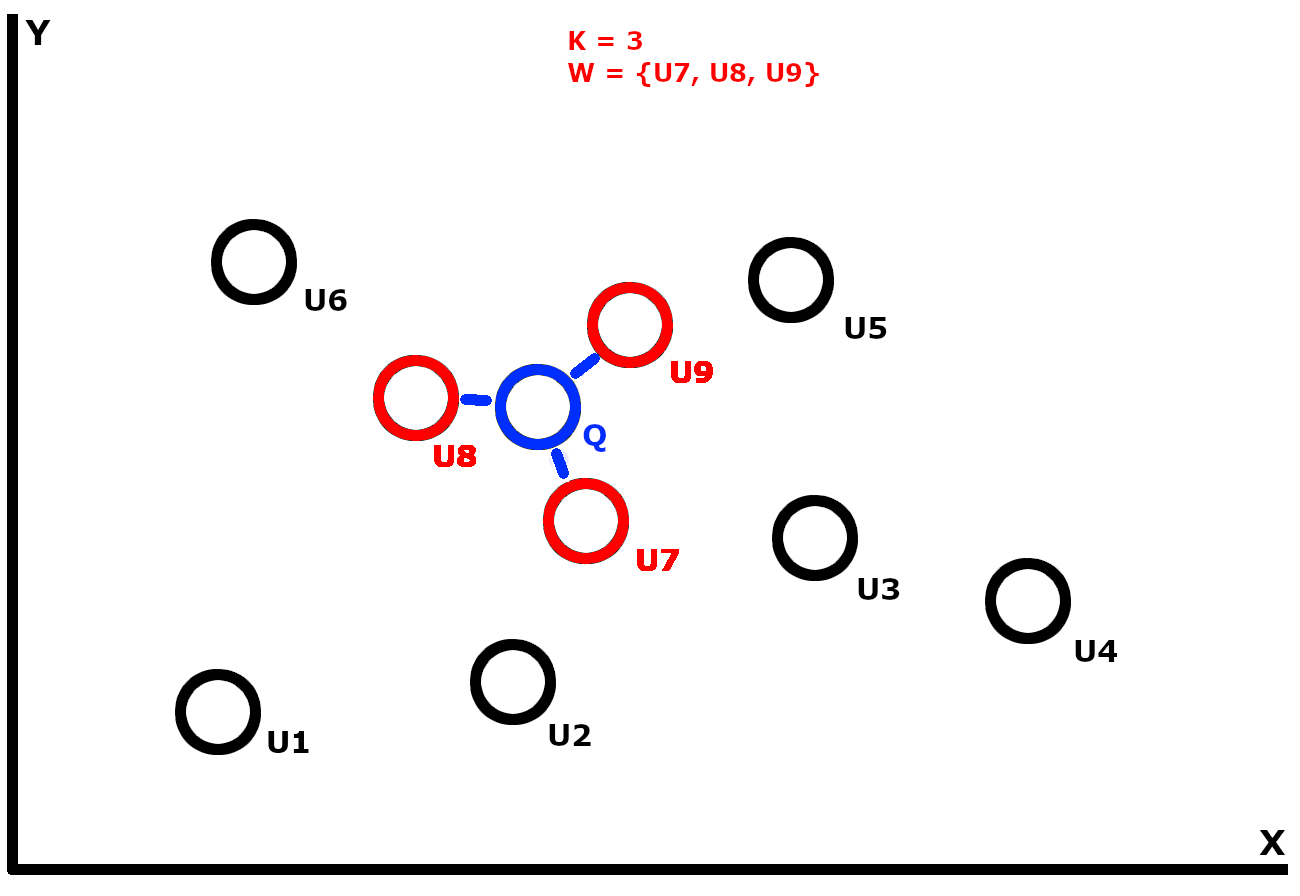
\includegraphics[scale=0.2]{figures/KNN_b3.jpg}
		\end{figure}
	\end{frame}

	\begin{frame}
		\frametitle{HNSW}
		
		\begin{itemize}
			\item Hierarchical Navigable Small Worlds
			\item Řešení KNN problému, přibližné vyhledávání s využitím vícevrstvých grafů
			\item Výsledek poskytován s určitou přesností zvanou Recall
			\item Přesnost se dá zvýšit navýšením hodnoty parametru Ef, stejně tak poroste ale i čas vykonání dotazu
		\end{itemize}
		
	\end{frame}

	\begin{frame}
		\frametitle{HNSW}
		
			\begin{figure}
			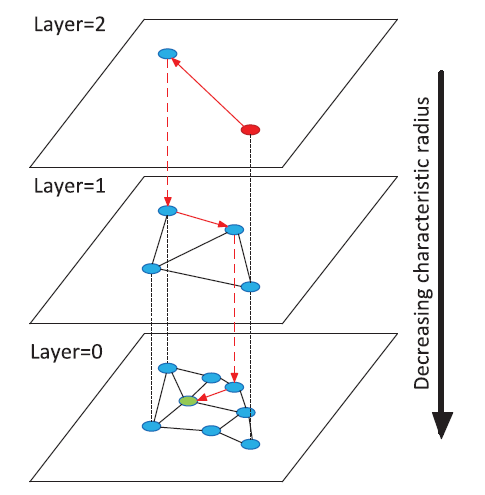
\includegraphics[scale=0.4]{figures/hnsw_layers.png}
			\caption{Vrstvy grafů v HNSW}
		\end{figure}
		
	\end{frame}

	\begin{frame}
		\frametitle{HNSW}
		
		\begin{figure}
			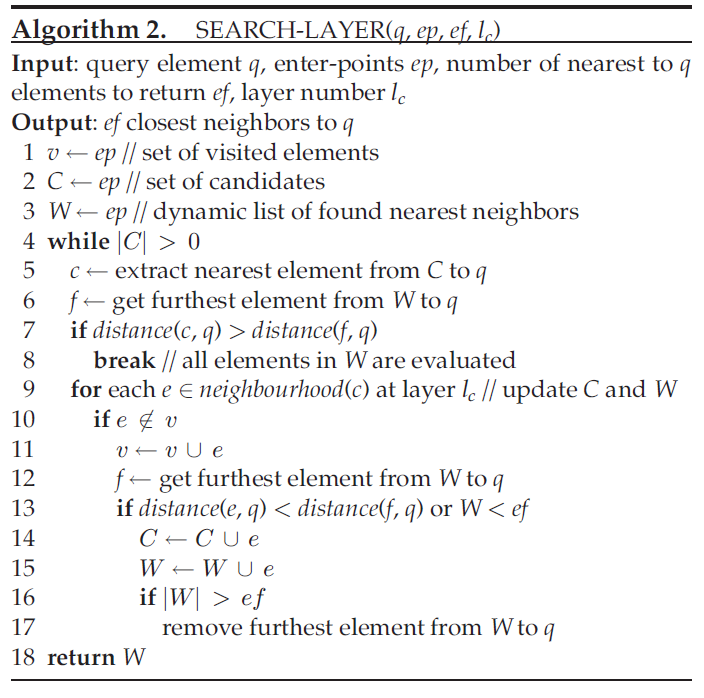
\includegraphics[scale=0.3]{figures/hnsw_search.png}
			\caption{Pseudokód HNSW Search algoritmu}
		\end{figure}
		
	\end{frame}

	\begin{frame}
		\frametitle{HNSW}
		
		\begin{figure}
			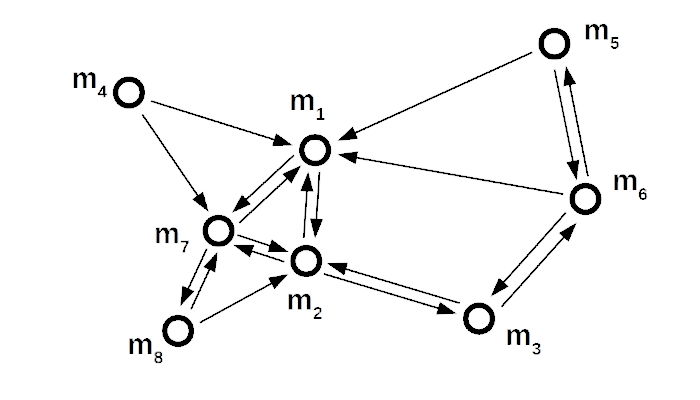
\includegraphics[scale=0.34]{figures/HNSW_b1.png}
		\end{figure}
		
	\end{frame}

	\begin{frame}
		\frametitle{HNSW}
		
		\begin{columns}[T] % align columns
			\begin{column}{.6\textwidth}
				\begin{figure}
					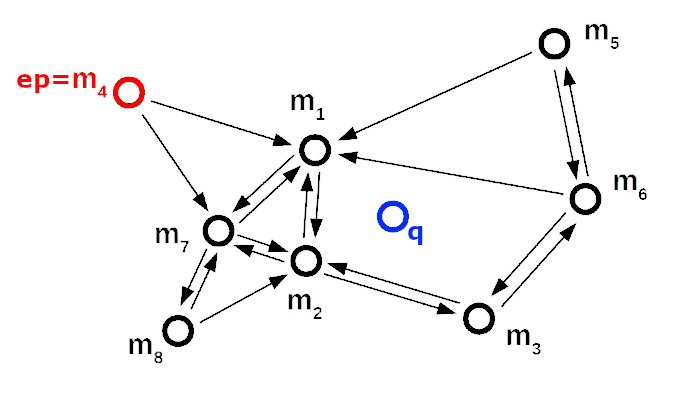
\includegraphics[scale=0.3]{figures/HNSW_b2.png}
				\end{figure}
			\end{column}%
			\hfill%
			\begin{column}{.4\textwidth}
				\begin{itemize}
					\item ep = \{m4\}
					\item[]
					\item V = \{m4\}
					\item[]
					\item W = \{m4\}
					\item C = \{m4\}
				\end{itemize}
			\end{column}%
		\end{columns}
		
	\end{frame}

	\begin{frame}
		\frametitle{HNSW}
		\begin{columns}[T] % align columns
			\begin{column}{.6\textwidth}
				\begin{figure}
					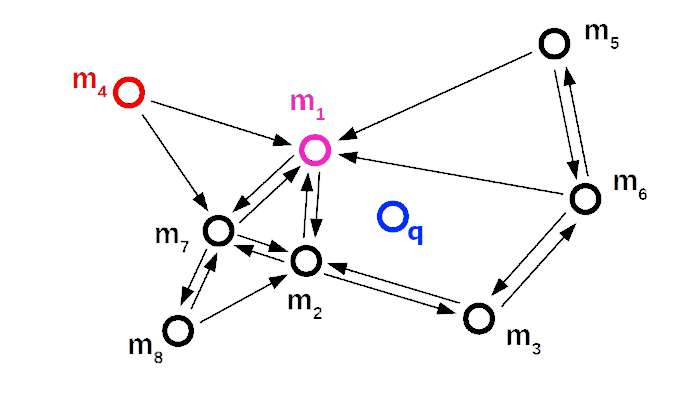
\includegraphics[scale=0.3]{figures/HNSW_b3.png}
				\end{figure}
			\end{column}%
			\hfill%
			\begin{column}{.4\textwidth}
				\begin{itemize}
					\item V = \{m4,m1\}
					\item[]
					\item W = \{m1,m4\}
					\item C = \{m1\}
					\item[]
					\item f = m4
					\item c = m4
				\end{itemize}
			\end{column}%
		\end{columns}
	\end{frame}

	\begin{frame}
		\frametitle{HNSW}
		\begin{columns}[T] % align columns
			\begin{column}{.6\textwidth}
				\begin{figure}
					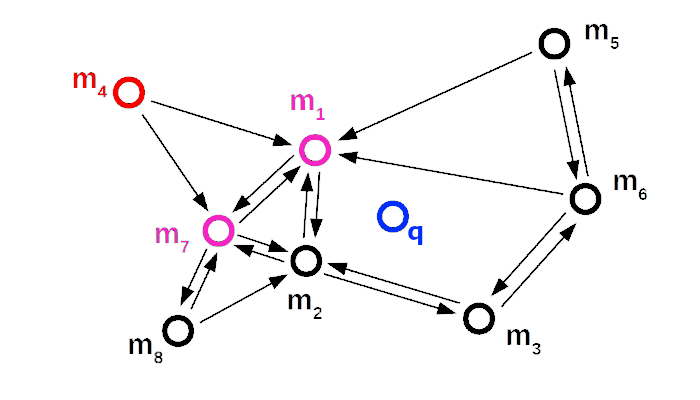
\includegraphics[scale=0.3]{figures/HNSW_b4.png}
				\end{figure}
			\end{column}%
			\hfill%
			\begin{column}{.4\textwidth}
				\begin{itemize}
					\item V = \{m4,m1,m7\}
					\item[]
					\item W = \{m1,m7,m4\}
					\item C = \{m1,m7\}
					\item[]
					\item f = m4
					\item c = m4
				\end{itemize}
			\end{column}%
		\end{columns}
	\end{frame}

	\begin{frame}
		\frametitle{HNSW}
		\begin{columns}[T] % align columns
			\begin{column}{.6\textwidth}
				\begin{figure}
					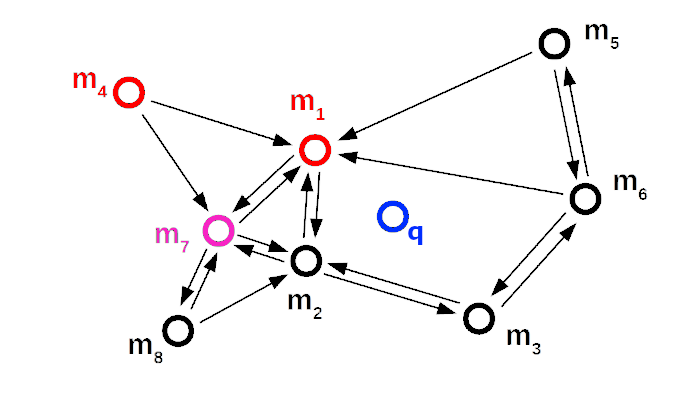
\includegraphics[scale=0.3]{figures/HNSW_b5.png}
				\end{figure}
			\end{column}%
			\hfill%
			\begin{column}{.4\textwidth}
				\begin{itemize}
					\item V = \{m4,m1,m7\}
					\item[]
					\item W = \{m1,m7,m4\}
					\item C = \{m7\}
					\item[]
					\item f = m4
					\item c = m1
				\end{itemize}
			\end{column}%
		\end{columns}
	\end{frame}

	\begin{frame}
		\frametitle{HNSW}
		\begin{columns}[T] % align columns
			\begin{column}{.6\textwidth}
				\begin{figure}
					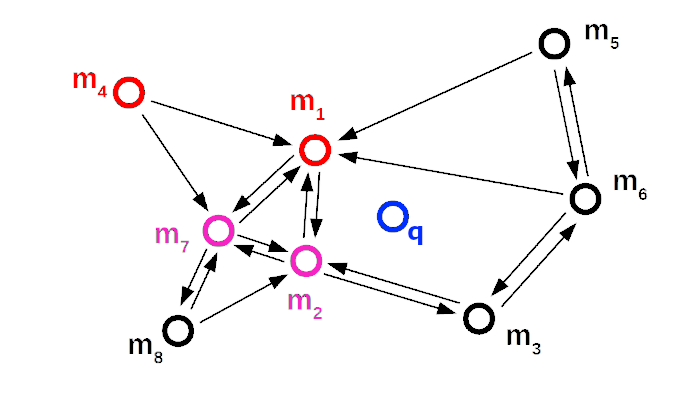
\includegraphics[scale=0.3]{figures/HNSW_b6.png}
				\end{figure}
			\end{column}%
			\hfill%
			\begin{column}{.4\textwidth}
				\begin{itemize}
					\item V = \{m4,m1,m7,m2\}
					\item[]
					\item W = \{m1,m2,m7\}
					\item C = \{m2,m7\}
					\item[]
					\item f = m7
					\item c = m1
				\end{itemize}
			\end{column}%
		\end{columns}
	\end{frame}

	\begin{frame}
		\frametitle{HNSW}
		\begin{columns}[T] % align columns
			\begin{column}{.6\textwidth}
				\begin{figure}
					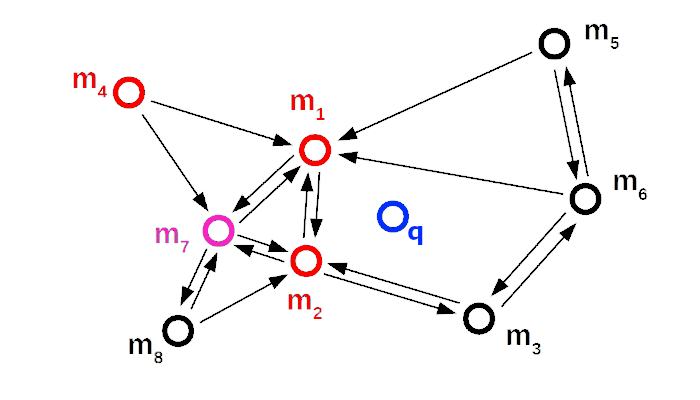
\includegraphics[scale=0.3]{figures/HNSW_b7.png}
				\end{figure}
			\end{column}%
			\hfill%
			\begin{column}{.4\textwidth}
				\begin{itemize}
					\item V = \{m4,m1,m7,m2\}
					\item[]
					\item W = \{m1,m2,m7\}
					\item C = \{m7\}
					\item[]
					\item f = m7
					\item c = m2
				\end{itemize}
			\end{column}%
		\end{columns}
	\end{frame}

	\begin{frame}
		\frametitle{HNSW}
		\begin{columns}[T] % align columns
			\begin{column}{.6\textwidth}
				\begin{figure}
					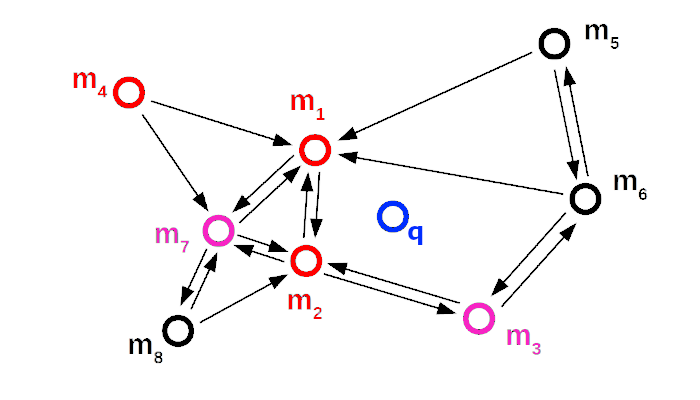
\includegraphics[scale=0.3]{figures/HNSW_b8.png}
				\end{figure}
			\end{column}%
			\hfill%
			\begin{column}{.4\textwidth}
				\begin{itemize}
					\item V = \{m4,m1,m7,m2,m3\}
					\item[]
					\item W = \{m1,m2,m3\}
					\item C = \{m3,m7\}
					\item[]
					\item f = m3
					\item c = m2
				\end{itemize}
			\end{column}%
		\end{columns}
	\end{frame}

	\begin{frame}
		\frametitle{HNSW}
		\begin{columns}[T] % align columns
			\begin{column}{.6\textwidth}
				\begin{figure}
					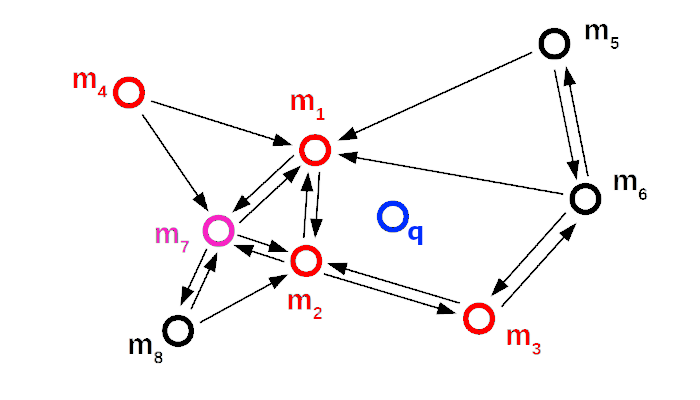
\includegraphics[scale=0.3]{figures/HNSW_b9.png}
				\end{figure}
			\end{column}%
			\hfill%
			\begin{column}{.4\textwidth}
				\begin{itemize}
					\item V = \{m4,m1,m7,m2,m3\}
					\item[]
					\item W = \{m1,m2,m3\}
					\item C = \{m7\}
					\item[]
					\item f = m3
					\item c = m3
				\end{itemize}
			\end{column}%
		\end{columns}
	\end{frame}

	\begin{frame}
		\frametitle{HNSW}
		\begin{columns}[T] % align columns
			\begin{column}{.6\textwidth}
				\begin{figure}
					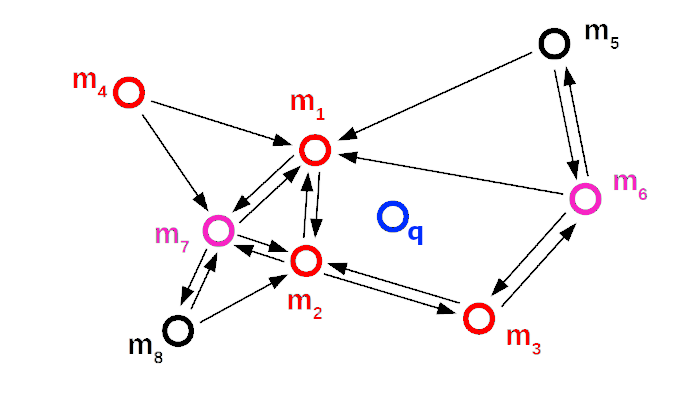
\includegraphics[scale=0.3]{figures/HNSW_b10.png}
				\end{figure}
			\end{column}%
			\hfill%
			\begin{column}{.4\textwidth}
				\begin{itemize}
					\item V = \{m4,m1,m7,m2,m3,m6\}
					\item[]
					\item W = \{m1,m2,m3\}
					\item C = \{m7,m6\}
					\item[]
					\item f = m3
					\item c = m3
				\end{itemize}
			\end{column}%
		\end{columns}
	\end{frame}

	\begin{frame}
		\frametitle{HNSW}
		\begin{columns}[T] % align columns
			\begin{column}{.6\textwidth}
				\begin{figure}
					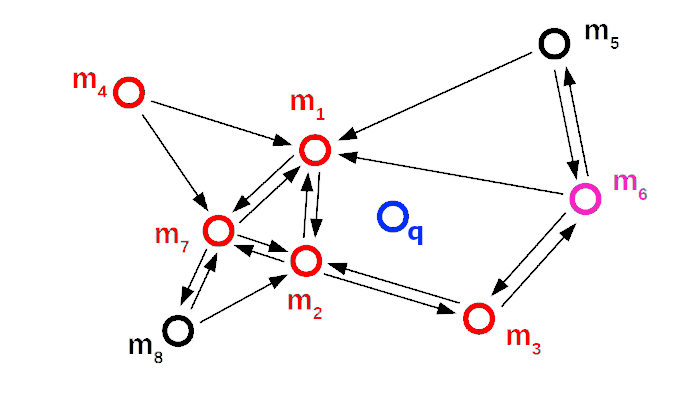
\includegraphics[scale=0.3]{figures/HNSW_b11.png}
				\end{figure}
			\end{column}%
			\hfill%
			\begin{column}{.4\textwidth}
				\begin{itemize}
					\item V = \{m4,m1,m7,m2,m3,m6\}
					\item[]
					\item W = \{m1,m2,m3\}
					\item C = \{m6\}
					\item[]
					\item f = m3
					\item c = m7
				\end{itemize}
			\end{column}%
		\end{columns}
	\end{frame}

	\begin{frame}
		\frametitle{HNSW}
		\begin{columns}[T] % align columns
			\begin{column}{.6\textwidth}
				\begin{figure}
					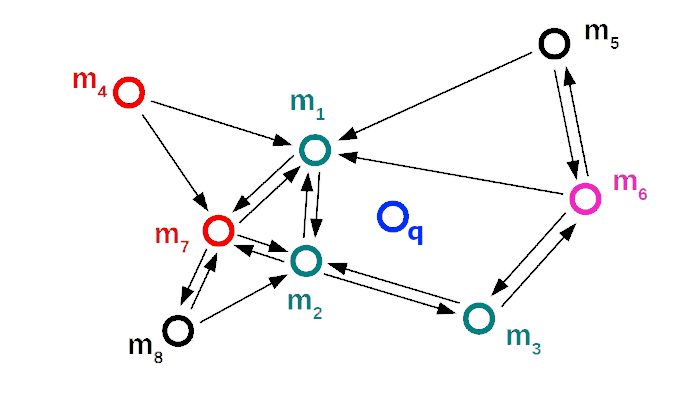
\includegraphics[scale=0.3]{figures/HNSW_b12.png}
				\end{figure}
			\end{column}%
			\hfill%
			\begin{column}{.4\textwidth}
				\begin{itemize}
					\item V = \{m4,m1,m7,m2,m3,m6\}
					\item[]
					\item \textcolor{teal}{W = \{m1,m2,m3\}}
					\item C = \{m6\}
					\item[]
					\item f = m3
					\item c = m7
					\item[]
					\item \textcolor{teal}{$dist(c,q) > dist(f,q)$}
				\end{itemize}
			\end{column}%
		\end{columns}
	\end{frame}
	
	\begin{frame}
		\frametitle{HNSW}
		
		\begin{figure}
			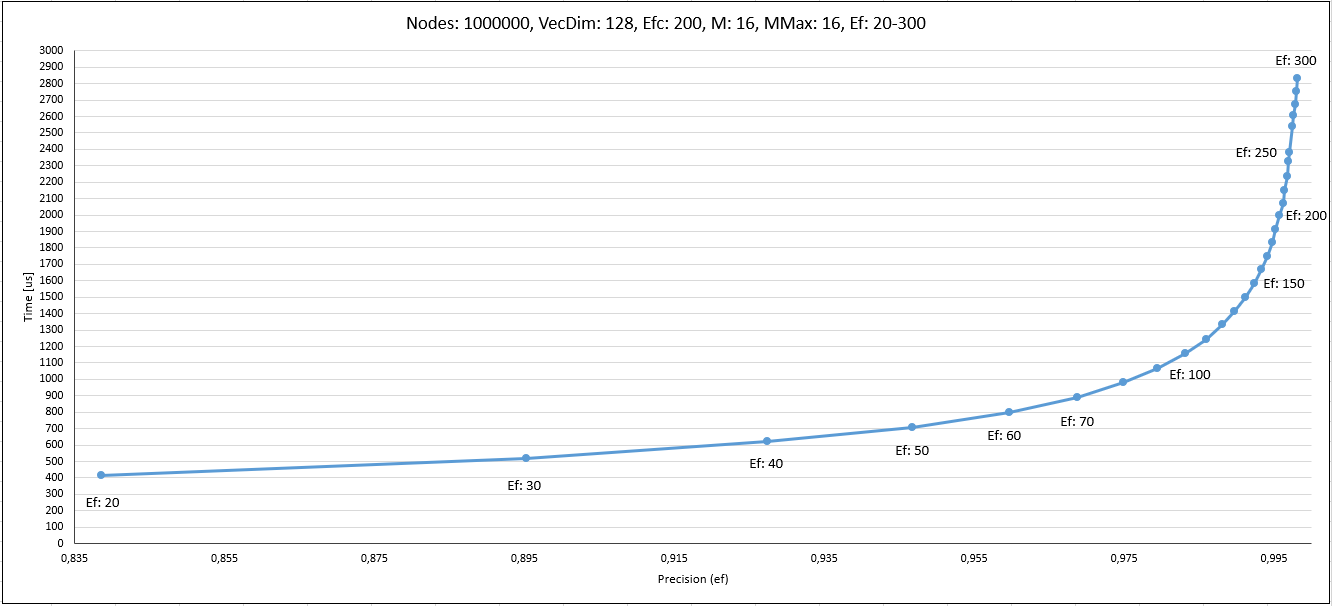
\includegraphics[scale=0.34]{figures/graf_hnsw.png}
			\caption{Graf závislosti průměrného času jednoho dotazu na přesnosti}
		\end{figure}
		
	\end{frame}
	
	\begin{frame}
		\frametitle{Filtr}
		
		\begin{itemize}
			\item Podmínka určující které vektory neprocházet a nevracet do výsledku
			\item Udává jakých hodnot mají nabývat jednotlivé atributy, nebo v jakých intervalech hodnot se mají nacházet
			\item Nemusíme omezovat všechny atribury
			\item Selektivita filtru $<0,1>$ udává procentuální počet uzlů z celé množiny všech uzlů, které filtr přijme
			
		\end{itemize}
		
	\end{frame}

	\begin{frame}
		\frametitle{Filtr}
		
		\begin{itemize}
			\item 72: $<51.32,143.87>$; 88: $<3>$; 110: $<72.40,106.84>$;
			\item[]
			\item vec[72] $\in$ $<51.32,143.87>$
			\item vec[88] = 3
			\item vec[110]  $\in$ $<72.40,106.84>$
		\end{itemize}
		
	\end{frame}

	\begin{frame}
		\frametitle{Filtr}
		\begin{columns}[T] % align columns
			
			\begin{column}{.6\textwidth}
				
				\begin{itemize}
					\item[] Filtr: vec[0] $\in$ $<50,100>$
				\end{itemize}
				
				\begin{figure}
					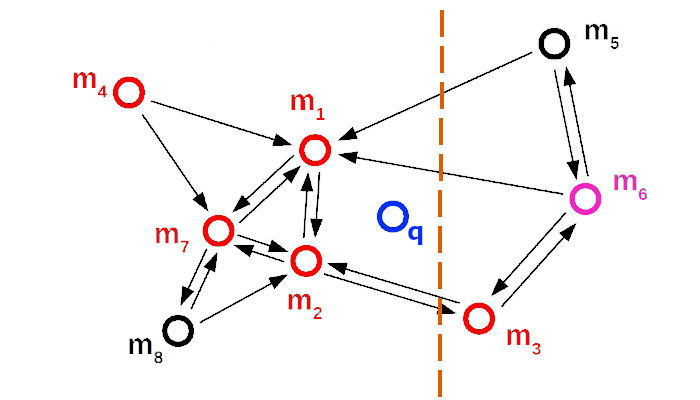
\includegraphics[scale=0.3]{figures/Filtry_b1.png}
				\end{figure}
			\end{column}%
			\hfill%
			\begin{column}{.4\textwidth}
				\begin{itemize}
					\item V = \{m4,m1,m7,m2,m3,m6\}
					\item[]
					\item W = \{m1,m2,m3\}
					\item C = \{m6\}
					\item[]
					\item f = m3
					\item c = m7
					\item[]
					\item $dist(c,q) > dist(f,q) $
				\end{itemize}
			\end{column}%
		\end{columns}
	\end{frame}

	\begin{frame}
		\frametitle{Filtr}
		\begin{columns}[T] % align columns
			
			\begin{column}{.6\textwidth}
				
				\begin{itemize}
					\item[] Filtr: vec[0] $\in$ $<50,100>$
				\end{itemize}
				
				\begin{figure}
					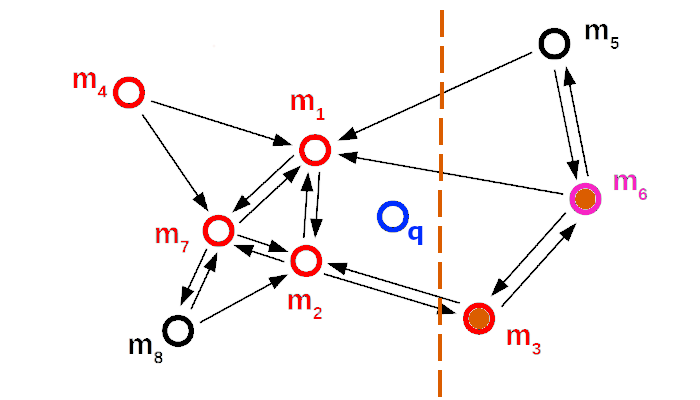
\includegraphics[scale=0.3]{figures/Filtry_b2.png}
				\end{figure}
			\end{column}%
			\hfill%
			\begin{column}{.4\textwidth}
				\begin{itemize}
					\item V = \{m4,m1,m7,m2,m3,m6\}
					\item[]
					\item F = \{m3,m6\}
					\item W = \{m1,m2,m3\}
					\item C = \{m6\}
					\item[]
					\item f = m3
					\item c = m7
					\item[]
					\item $dist(c,q) > dist(f,q)$
					\item $|F| == K$
				\end{itemize}
			\end{column}%
		\end{columns}
	\end{frame}

	\begin{frame}
		\frametitle{Filtr}
		\begin{columns}[T] % align columns
			\begin{column}{.6\textwidth}
				\begin{itemize}
					\item[] Filtr: vec[0] $\in$ $<50,100>$
				\end{itemize}
				
				\begin{figure}
					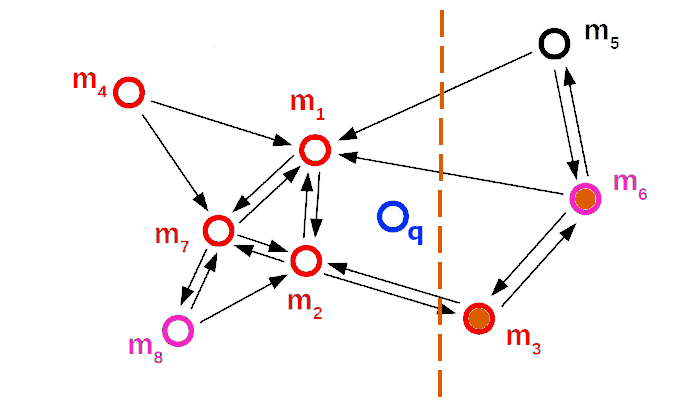
\includegraphics[scale=0.3]{figures/Filtry_b3.png}
				\end{figure}
			\end{column}%
			\hfill%
			\begin{column}{.4\textwidth}
				\begin{itemize}
					\item V = \{m4,m1,m7,m2,m3,m6, m8\}
					\item[]
					\item F = \{m3,m6\}
					\item W = \{m1,m2,m3\}
					\item C = \{m6,m8\}
					\item[]
					\item f = m3
					\item c = m7
				\end{itemize}
			\end{column}%
		\end{columns}
	\end{frame}

	\begin{frame}
		\frametitle{Filtr}
		\begin{columns}[T] % align columns
			\begin{column}{.6\textwidth}
				\begin{itemize}
					\item[] Filtr: vec[0] $\in$ $<50,100>$
				\end{itemize}
				\begin{figure}
					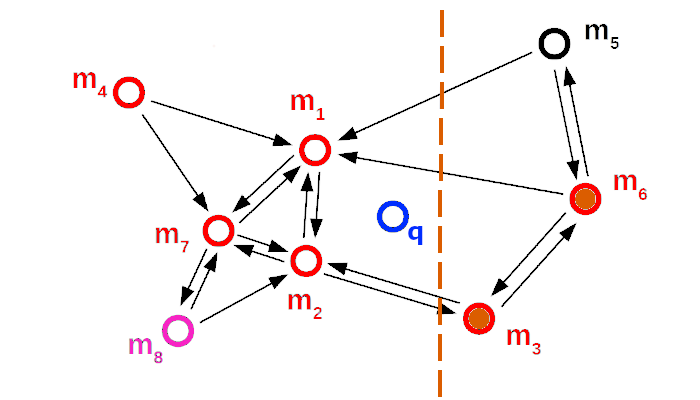
\includegraphics[scale=0.3]{figures/Filtry_b4.png}
				\end{figure}
			\end{column}%
			\hfill%
			\begin{column}{.4\textwidth}
				\begin{itemize}
					\item V = \{m4,m1,m7,m2,m3,m6, m8\}
					\item[]
					\item F = \{m3,m6\}
					\item W = \{m1,m2,m3\}
					\item C = \{m8\}
					\item[]
					\item f = m3
					\item c = m6
				\end{itemize}
			\end{column}%
		\end{columns}
	\end{frame}

	\begin{frame}
		\frametitle{Filtr}
		\begin{columns}[T] % align columns
			\begin{column}{.6\textwidth}
				\begin{itemize}
					\item[] Filtr: vec[0] $\in$ $<50,100>$
				\end{itemize}
				\begin{figure}
					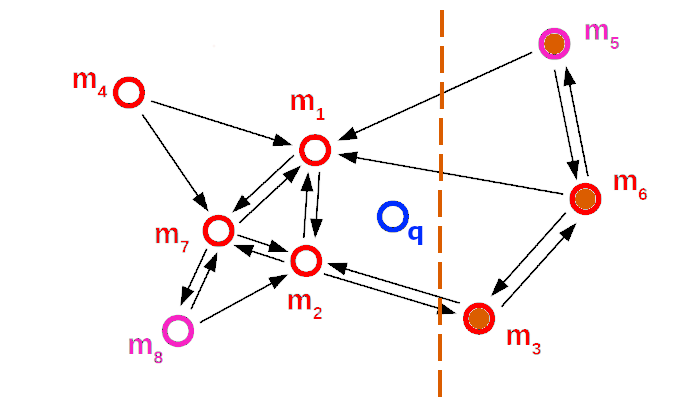
\includegraphics[scale=0.3]{figures/Filtry_b5.png}
				\end{figure}
			\end{column}%
			\hfill%
			\begin{column}{.4\textwidth}
				\begin{itemize}
					\item V = \{m4,m1,m7,m2,m3,m6, m8,m5\}
					\item[]
					\item F = \{m3,m6,m5\}
					\item W = \{m1,m2,m3\}
					\item C = \{m5,m8\}
					\item[]
					\item f = m3
					\item c = m6
				\end{itemize}
			\end{column}%
		\end{columns}
	\end{frame}

	\begin{frame}
		\frametitle{Filtr}
		\begin{columns}[T] % align columns
			\begin{column}{.6\textwidth}
				\begin{itemize}
					\item[] Filtr: vec[0] $\in$ $<50,100>$
				\end{itemize}
				\begin{figure}
					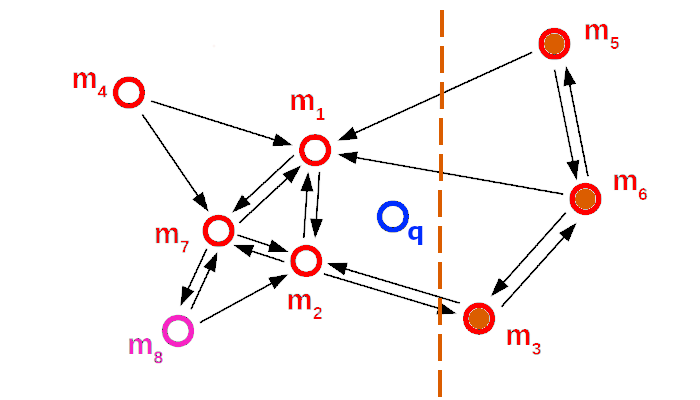
\includegraphics[scale=0.3]{figures/Filtry_b6.png}
				\end{figure}
			\end{column}%
			\hfill%
			\begin{column}{.4\textwidth}
				\begin{itemize}
					\item V = \{m4,m1,m7,m2,m3,m6, m8,m5\}
					\item[]
					\item F = \{m3,m6,m5\}
					\item W = \{m1,m2,m3\}
					\item C = \{m8\}
					\item[]
					\item f = m3
					\item c = m5
				\end{itemize}
			\end{column}%
		\end{columns}
	\end{frame}

	\begin{frame}
		\frametitle{Filtr}
		\begin{columns}[T] % align columns
			\begin{column}{.6\textwidth}
				\begin{itemize}
					\item[] Filtr: vec[0] $\in$ $<50,100>$
				\end{itemize}
				\begin{figure}
					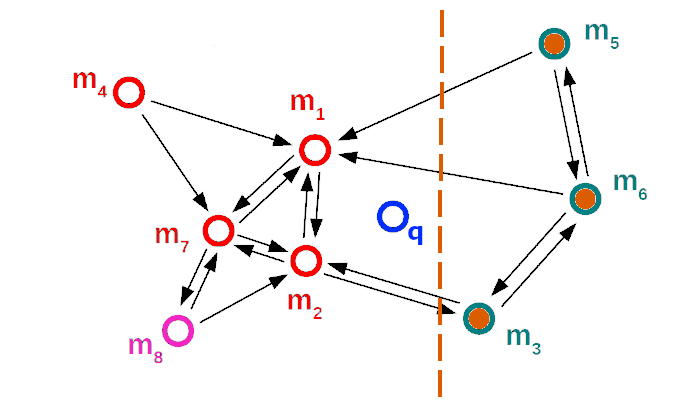
\includegraphics[scale=0.3]{figures/Filtry_b7.png}
				\end{figure}
			\end{column}%
			\hfill%
			\begin{column}{.4\textwidth}
				\begin{itemize}
					\item V = \{m4,m1,m7,m2,m3,m6, m8,m5\}
					\item[]
					\item \textcolor{teal}{F = \{m3,m6,m5\}}
					\item W = \{m1,m2,m3\}
					\item C = \{m8\}
					\item[]
					\item f = m3
					\item c = m5
					\item[]
					\item \textcolor{teal}{$dist(c,q) > dist(f,q)$}
					\item \textcolor{teal}{$|F| == K$}
				\end{itemize}
			\end{column}%
		\end{columns}
	\end{frame}

	\begin{frame}
		\frametitle{Filtr}
		
		\begin{figure}
			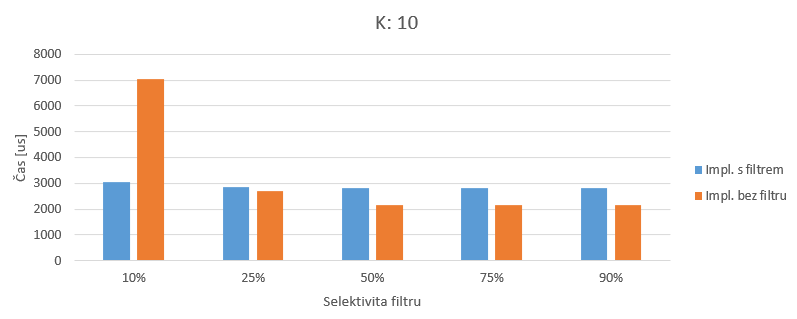
\includegraphics[scale=0.4]{figures/graf_filtr_k10.png}
		\end{figure}
	
		\begin{figure}
			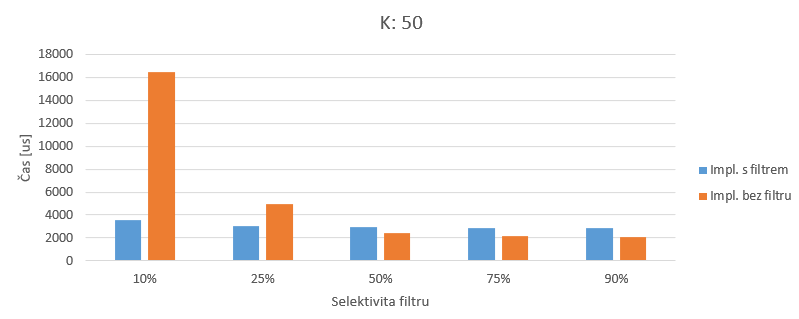
\includegraphics[scale=0.4]{figures/graf_filtr_k50.png}
		\end{figure}
		
	\end{frame}

	\begin{frame}
		\frametitle{Filtr}
		
		\begin{figure}
			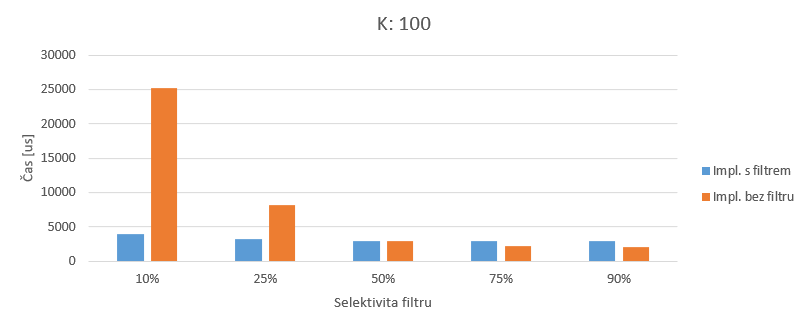
\includegraphics[scale=0.4]{figures/graf_filtr_k100.png}
		\end{figure}
		
		\begin{figure}
			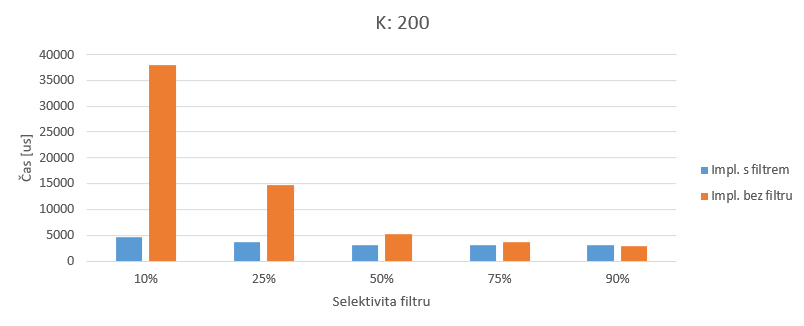
\includegraphics[scale=0.4]{figures/graf_filtr_k200.png}
		\end{figure}
		
	\end{frame}

	\begin{frame}
		\frametitle{Závěr}
		
		\begin{itemize}
			\item Splnění všech požadavků
			\item Funkční implementace původního HNSW
			\item HNSW implementace o polovinu pomalejší než reference
			\item Funkční implementace rozšířeného HNSW o filtry
		\end{itemize}
		
	\end{frame}

	\begin{frame}
		\frametitle{Poděkování}
		
		\begin{center}
			\Huge
			Děkuji za pozornost
		\end{center}
		
	\end{frame}

	\begin{frame}[noframenumbering,allowframebreaks]
		\frametitle{Citace}
		
		\nocite{*}
		
		\printbibliography
		
	\end{frame}
	
\end{document}